\begin{recipe}{Rotoli di pollo con verdure -- Jawad}
    \begin{header}
        \portion{3}[rotoli]
        \source{Jawad Shurrush}
        \recipedate{2022}

        \preparationTime     {\timeH{1}}
        \cookingTime         {\timeM{15}}{Fiamma media}
        \bakingTimeTopbottom {\timeM{30-40}}{200}[Vedere cottura pasta sfoglia]
    \end{header}
    
    \begin{ingredients}[15]
        \ingredientSection*{Verdure}
        \ingredient[100][g]{Cipolle}
        \ingredient[150][g]{Peperone rosso}
        \ingredient[150][g]{Peperone giallo}
        \ingredient[300][g]{Mais}

        \ingredientSection{Pollo}
        \ingredient[700][g]{Petto di pollo}
        \ingredient{Olio}

        \ingredientSection{Spezie}
        \ingredient{Sale}
        \ingredient{Pepe}
        \ingredient{Pepe inglese}
        \ingredient{Cannella}
        \ingredient{Noce moscata}
        \ingredient[80][ml]{Salsa di soia}
        
        \ingredientSection{Impasto}
        \ingredient[3][rotoli]{Pasta sfoglia}
        \ingredient[3-5]{Tuorli}
        \ingredient{Sesamo}
    \end{ingredients}
    
    \begin{preparation}
        \step Tagliare verdure e pollo a cubetti (circa \sfrac{1}{2} cm).
        \step Iniziare a soffriggere cipolla in una padella, pollo (e olio) in un'altra.
        
        \step Quando le verdure iniziane ad essere soffritte, aggiungere peperoni.
        \step Quando le verdure sono quasi completamente soffritte, aggiungere mais (circa \timeM{1} prima che siano pronte).

        \step Quando il pollo ha preso colore, aggiungere spezie.

        \step Quando le due padelle sono pronte, aggiungere (in entrambe) salsa di soia. Nel pollo ci andrà più salsa rispetto alle verdure.
        \step Cuocere entrambe per \timeM{5}.
        
        \step Unire verdure e pollo e regolare con il sale.

        \step*
        \step*
        
        \step Disporre il preparato sulla pasta sfoglia e richiudere
            \textit{(tagliare la pasta sfoglia come illustrato in figura \ref{fig:pollo_jawad:tagli_pasta_sfoglia})}.
        \step Spennellare con i tuorli e cospargere di sesamo.
        \step Infornare.
        \step Una volta pronto, tagliare a fette da un paio di cm.
    \end{preparation}

    \newpage
    \begin{figure}[h]
        \centering
        
        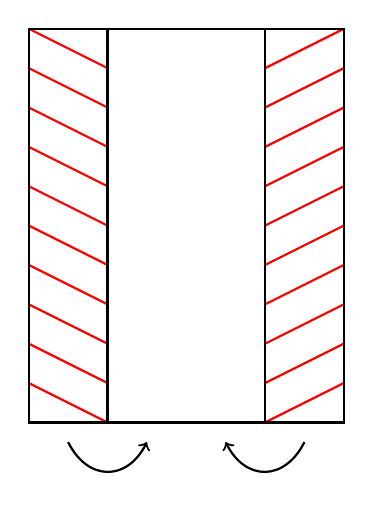
\begin{tikzpicture}[scale=1,
            color=black, fill=black!10, thick,
            cut/.style={color=red}
        ]
            \draw[cut] (0,5.0) -- (1,4.5);
            \draw[cut] (0,4.5) -- (1,4.0);
            \draw[cut] (0,4.0) -- (1,3.5);
            \draw[cut] (0,3.5) -- (1,3.0);
            \draw[cut] (0,3.0) -- (1,2.5);
            \draw[cut] (0,2.5) -- (1,2.0);
            \draw[cut] (0,2.0) -- (1,1.5);
            \draw[cut] (0,1.5) -- (1,1.0);
            \draw[cut] (0,1.0) -- (1,0.5);
            \draw[cut] (0,0.5) -- (1,0.0);

            \draw[cut] (3,4.5) -- (4,5.0);
            \draw[cut] (3,4.0) -- (4,4.5);
            \draw[cut] (3,3.5) -- (4,4.0);
            \draw[cut] (3,3.0) -- (4,3.5);
            \draw[cut] (3,2.5) -- (4,3.0);
            \draw[cut] (3,2.0) -- (4,2.5);
            \draw[cut] (3,1.5) -- (4,2.0);
            \draw[cut] (3,1.0) -- (4,1.5);
            \draw[cut] (3,0.5) -- (4,1.0);
            \draw[cut] (3,0.0) -- (4,0.5);

            % box - needs to be drawn on top of red lines
            \draw (0,0) -- (4,0) -- (4,5) -- (0,5) -- cycle;
            \draw (1,0) -- (1,5);
            \draw (3,0) -- (3,5);

            \draw[->] (0.5,-0.25) .. controls (.75, -.75) and (1.25, -.75) .. (1.5, -0.25);
            \draw[->] (3.5,-0.25) .. controls (3.25, -.75) and (2.75, -.75) .. (2.5, -0.25);

            % \filldraw (-.5,0.1) .. controls (-2, 2) and (-2, 3) .. (-.5, 4.9) -- cycle;
            % \filldraw (4.5,0.1) .. controls (6, 2) and (6, 3) .. (4.5, 4.9) -- cycle;
        \end{tikzpicture}
        
        \caption{Tagliare la pasta sfoglia lungo le linee rosse.}
        \label{fig:pollo_jawad:tagli_pasta_sfoglia}
    \end{figure}
\end{recipe}
